\chapter{Część przeglądowa}

\begin{itemize}
	\item JSON \cite{JSON} (JavaScript Object Notation) - jest to tekstowy format wymiany danych, bazującym na podzbiorze języka JavaScript. JSON przechowuje dane określone przez standard ECMA-262 3-cia edycja - Grudzień 1999.
	\item Transpilacja \cite{Transpilator} - Transpilatory lub kompilatory typu źródło-źródło to narzędzia, które odczytują kod źródłowy napisany w jednym języku programowania i wytwarzają równoważny kod w innym języku. Języki, które piszesz, które są transpilowane na JavaScript, są często nazywane językami kompilacji do JS i mówi się, że są ukierunkowane na JavaScript.
	\item SPA \cite{SPA} (także Single Page Application) - jednostronna aplikacja internetowa, czyli taka, która posiada tylko jeden plik HTML. Taka aplikacja nie przeładowuje strony w trakcie użytkowania. Może w tym celu korzystać z technologii AJAX lub innych dostępnych w przeglądarkach internetowych. Logika aplikacji SPA napisana jest w JavaScript lub w języku transpilowanym do języka JavaScript Framework.
\end{itemize}


\section{Słowniczek Pojęć}

\section{Przegląd prac o podobnej tematyce}

W części tej zajmiemy się przeglądem dostępnych rozwiązań oraz prac dotyczących pomiaru wydajności aplikacji internetowych z naciskiem na aplikacje typu SPA.

\subsection{Comparison of Single-Page Application Frameworks}

Pierwszą pozycją jest praca autorstwa Pan Eric'a Molina z instytutu KTH Royal Institute of Technology w Sztokholmie \cite{Molin}.
Autor stara się porównać frameworki na pełnej płazczyźnie ich złożoności.
W jego pracy znaleźć możemy pełen spis kryteriów oceny frameworków wraz z wagami przypisanymi do cech określonymi za pomocą wywiadu środowiskowego jaki autor przeprowadził na grupie 10 profesjonalnych deweloperów mających doświadczenie w tych zagadnieniach przedstawionych na rysunku \ref{fig:rysunek_1}.

\begin{figure}[!ht]
    \centering
    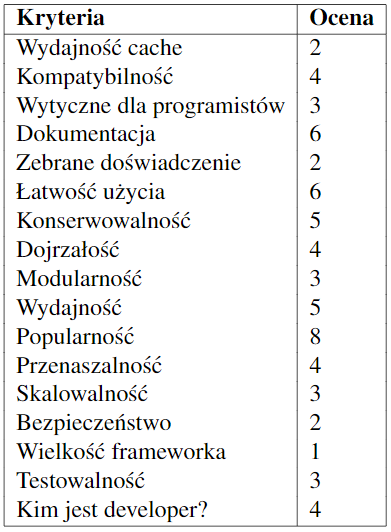
\includegraphics[width=12cm]{rysunek_1.png}
    \caption{Grafika przedstawiająca ocenę wpływu wybranego elementu na atrakcyjność danego narzędzia \cite{Molin}}
    \label{fig:rysunek_1}
\end{figure}




W pracy tej, porównywanymi frameworkami są AngularJS, Angular2 oraz React.
I tutaj wyróżnić możemy już pierwsze różnice pomiędzy pracami. Praca Pana Molina została wykonana w 2016 roku.
JavaScript jest jednym z najszybciej rozwijających  się oraz najczęściej spotykanych technologii webowych na świecie \cite{octoverse}.
Przez okres 4 lat, firmy masowo porzuciły technologie AngularJS na rzecz Angular 2 oraz Reacta.
Dodatkowo, w między czasie do wyścigu dołączył Vue.Js \cite{vue}.
Przez ten okres, także implementacja tychże rozwiązań znacznie dojrzała.
Angular z wersji 2 ewoluował już do wersji 9 \cite{angular-changelog}.
Także React ewoluował z wersji 0.14.8 (użyta w pracy  Pana Molina) do wersji 16.13.1 \cite{react-changelog}.
Najważniejszą zmianą którą należy tutaj wspomnieć jest zmiana silnika reacta nosząca nazwę React Fiber która nastąpiła w wersji 16.0.0.
Był to kamień milowy, i z punktu widzenia badania wydajności, jest to całkowicie nowe rozwiązanie. 

Następną sekcją która jest dla nas interesująca jest sekcja 5.2 w której autor prezentuje wyniki swoich testów.
Wartym zauważenia jest wersja przeglądarki chrome, która wynosi 50.0.26661.102m.
Najnowsza wersja chrome, w czasie pisania tego tekstu, to wersja \textit{80.0.3987.16} czyli aż o 30 wersji nowszej. 

W pierwszym teście, autor porównuje wydajność pomiędzy rozwiązaniami na przykładzie ładowania elementów od 10 aż do 5000 przedstawionym na rysunku \ref{fig:rysunek_2}.

\begin{figure}[!ht]
    \centering
    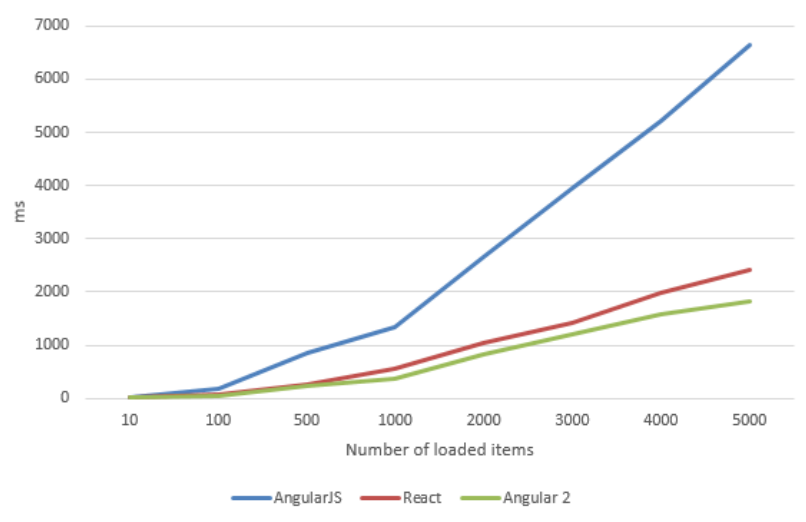
\includegraphics[width=12cm]{rysunek_2.png}
    \caption{Grafika przedstawiająca wzrost czasu ładowania elementów od 10 do 5000 przy użyciu AngularJS Angular2 oraz React \cite{Molin}}
    \label{fig:rysunek_2}
\end{figure}

Z badania tego, możemy zauważyć jak bardzo AngularJS różni się od pozostałych, nowszych rozwiązań. Do pierwszych 100 elementów, wyniki są zbliżone, natomiast powyżej tej wartości, mamy nagłą zmianę stopnia nachylenia funkcji. Przyczyną takiego zachowania jest fakt, iż AngularJS nigdy nie był zoptymalizowany dla takich przypadków użycia podczas, gdy React oraz Angular2 już tak.
W drugim teście, autor bada czas potrzebny do załadowania określonej ilości elementów. Wyniki przedstawiono na rysunku \ref{fig:rysunek_3}.

\begin{figure}[!ht]
    \centering
    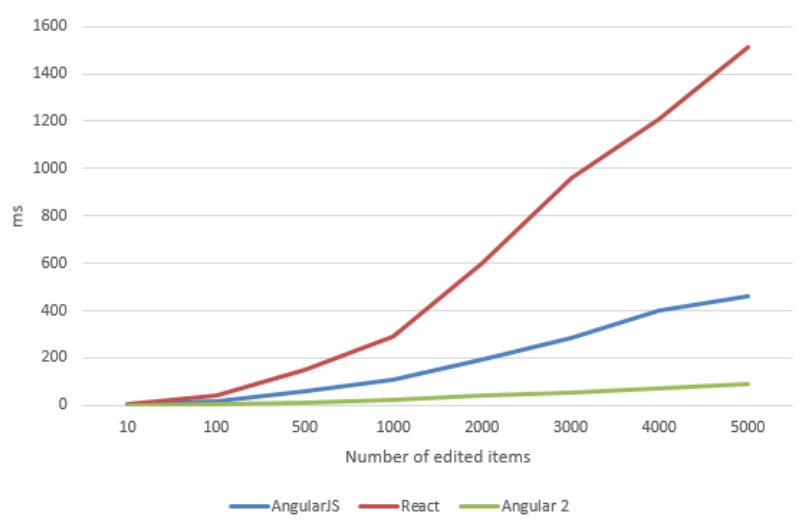
\includegraphics[width=12cm]{rysunek_3.png}
    \caption{Grafika przedstawiająca wykres zależności czasu do ilości edytowanych elementów na stronie \cite{Molin}}
    \label{fig:rysunek_3}
\end{figure}

Widzimy znaczną dysproporcję pomiędzy każdym z rozwiązań. Z jednej strony AngularJS przypomina funkcję wykładniczą gdzie po przeciwnej stronie Angular2 zachowuje się jak funkcja liniowa. Pokazuje to jak bardzo istotne zmiany zaszły pomiędzy zmianą generacji oraz wpływ doświadczenia jakie zebraliśmy w okresie panowania frameworka AngularJS. Wszak AngularJS był pierwszym podejściem do generycznego narzędzia dla dynamicznych aplikacji internetowych.
W ostatnim teście wydajnościowym, autor porównuje czas ładowania się aplikacji. Wyniki przedstawiono na rysunku \ref{fig:rysunek_4}.

\begin{figure}[!ht]
    \centering
    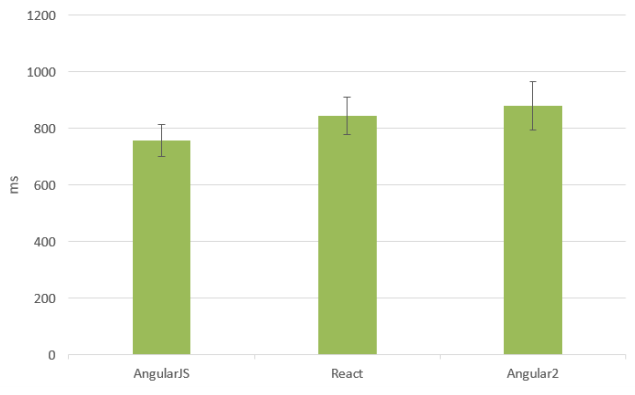
\includegraphics[width=12cm]{rysunek_4.png}
    \caption{Grafika przedstawiająca wykres czasu ładowania aplikacji \cite{Molin}}
    \label{fig:rysunek_4}
\end{figure}

O ile autor faktycznie porównuje wydajność rozwiązań, nie określa on w sposób klarowny jak zaimplementowano mechanizm dodawania oraz aktualizacji elementów w pierwszym oraz drugim teście.
Są to informacje bardzo istotne, gdyż każdy z frameworków działa w inny sposób, i ma to bezpośredni wpływ na otrzymane wyniki.
Dodatkowo, autor nie podaje błędu pomiaru \cite{probalistyka} który wyznaczył podczas przeprowadzania badania.
Jest to bardzo istotna informacja, gdyż frameworki takie opierają się na całej piramidzie warstw oprogramowania które współdzielą zasoby komputera z innymi procesami.
Ponadto auto nie zastosował żadnej warstwy abstrakcji nad systemem operacyjnym co powoduje, że wyniki mogą znacząco różnić się pomiędzy różnymi wersjami systemu.

\subsection{Lighthouse}

Jest to narzędzie open-source stworzone przez firmę Google do badania wydajności stron internetowych oraz aplikacji webowych \cite{lighthouse}. Jest ono integralną częścią przeglądarki Chrome, tak więc jest ono niezwykle łatwe w użytkowaniu. Narzędzie to pozwala nam na ocenę naszej aplikacji w kilku wybranych kategoriach w tym wydajności. Dodatkowo, narzędzie pozwala nam na określenie trybu badania gdzie do wyboru mamy tryb mobilny oraz tryb użytkownika komputera domowego. Ma to bardzo duży wpływ na wynik testu, gdyż wydajność urządzeń mobilnych jest z reguły bardzo ograniczona w porównaniu do pełnoprawnej platformy domowej. Metrykami jakie możemy otrzymać to:
\begin{itemize}
	\item Czas rozpoczęcia pierwszego renderowania
	\item Czas gdy strona faktycznie została wyrenderowana w całości
	\item Indeks szybkości - czas, gdy główna treść strony została wyrenderowana
	\item Czas do interakcji - czyli czas, gdy użytkownik faktycznie może zacząć interakcję ze stroną
\end{itemize}

Jednak o ile informacje te są jak najbardziej przydatne z punktu widzenia ładowania strony,
narzędzie to nie jest w stanie określić faktycznego czasu interakcji ze stroną.
Wpływ na taki czas ma wiele czynników z których najważniejszym jest ilość elementów na stronie.
Jest to istotne, gdyż JavaScript jest językiem jednowątkowym z mechanizmem event loop \cite{you-dont-know-js}.
Tak więc jesteśmy w stanie otrzymać informacje o wydajności ładowania aplikacji przez przeglądarkę,
jednak narzędzie w żaden sposób nie wspiera pomiarów działania aplikacji po etapie ładowania, a właśnie na tym skupia się ta praca.

\subsection{Porównanie narzędzi do tworzenia aplikacji typu SPA na przykładzie Angular2 i React}

Praca Pań Jadwiga Kalinowska oraz Beata Pańczyk \cite{polibuda} także ma na celu porównanie aplikacja typu SPA, tym razem Angular2 oraz React.
Autorzy przedstawiają szereg metryk według których porównywać będą obydwa narzędzia.
Pierwszą metryką jest sama struktura aplikacji czyli jak wygląda architektura wewnętrzna rozpatrywanego frameworka.
I jak autorki trafnie zauważają, obydwa rozwiązania czerpią garściami z nowoczesnej szkoły tworzenia wysoce skalowalnych i wydajnych rozwiązań implementując naturę tworzenia złożonych aplikacji z małych komponentów.
Z komponentów takich składamy coraz to większą i bardziej złożoną aplikację.
Drugą metryką rozpatrywaną przez autorki jest metryka kodu przedstawiona na rysunku \ref{fig:rysunek_5}.
Innymi słowy, jak wiele kodu boilerplate należy napisać, aby osiągnąć ten sam efekt.
Ma to wpływ przede wszystkim na końcowy rozmiar pliku który należy przesłać pomiędzy serwerem a klientem.
Im niższa wartość, tym lepiej.

\begin{figure}[!ht]
    \centering
    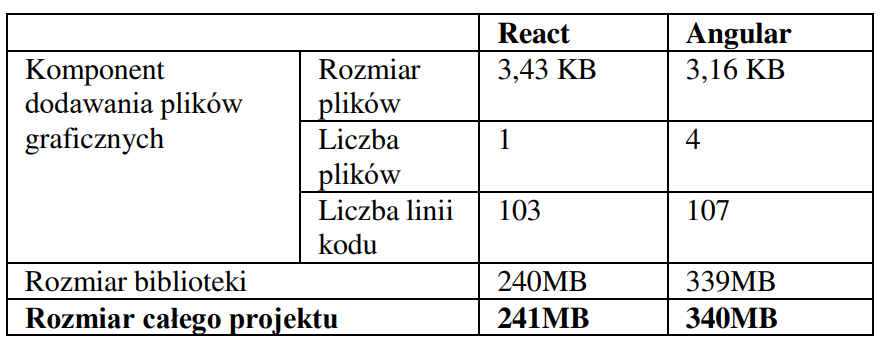
\includegraphics[width=12cm]{rysunek_5.png}
    \caption{Porównanie metryk kodu dla pojedynczego komponentu \cite{polibuda}}
    \label{fig:rysunek_5}
\end{figure}

Wnioskiem płynącym z otrzymanych danych jest fakt, iż React jest finalnie znacznie mniejszym frameworkiem co bezpośrednie redukuje koszt wytworzenia oraz utrzymania kodu.
Ostatnim interesującym punktem jest metryka badająca bezpośrednią wydajność aplikacji przedstawiona na rysunku \ref{fig:rysunek_6}.
Badanie miało na celu zmierzenie czasu, jaki potrzebny jest aby pobrać rekordy z przygotowanej bazy danych.

\begin{figure}[!ht]
    \centering
    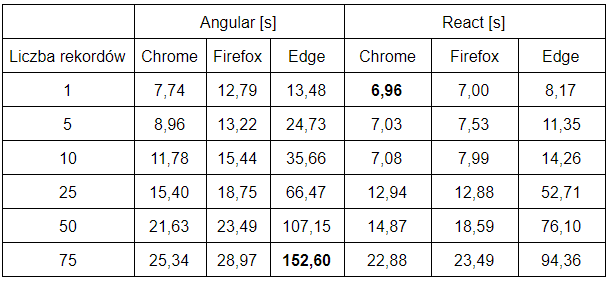
\includegraphics[width=12cm]{rysunek_6.png}
    \caption{Porównanie czasów pobrania danych z bazy \cite{polibuda}}
    \label{fig:rysunek_6}
\end{figure}

Interesującym wynikiem jest fakt, iż React w przeglądarce Google Chrome dla 1,5 oraz 10 wyników otrzymał bardzo zbliżone czasy bliskie błędowi pomiaru.
Jednak im większa liczba rekordów pobrana z bazy, tym większą przewagę osiągał React. 
Wszystkie metryki które zostały zastosowane podczas porównania dobrze obrazują różnicę pomiędzy tymi rozwiązaniami, ale tylko w ujęciu wysoko poziomowym.
Badanie zawiera w sobie serwer WWW oraz bazę danych, których czasy stanowią znaczną część czasu uzyskanego w wynikach.
Nie pozwala to nam na jednoznaczne stwierdzenie, które narzędzie jest wydajniejsze, gdyż wykonano tylko jedno badanie, które nie pozwala na ocenę tych narzędzi pod kątem różnych przypadków użycia.
